% !TEX TS-program = pdflatex
\documentclass[11pt]{article}

% -------------------- Packages --------------------
\usepackage[a4paper,margin=1in]{geometry}
\usepackage{amsmath,amssymb}
\usepackage[T1]{fontenc}
\usepackage{lmodern}
\usepackage{xcolor}
\usepackage{tcolorbox}
\tcbuselibrary{skins,breakable}
\usepackage{enumitem}
\usepackage{hyperref}

% --- Tables & Diagrams ---
\usepackage{booktabs}
\usepackage{array}
\usepackage{colortbl}
\usepackage{tikz}
\usepackage{pgfplots}
\pgfplotsset{compat=1.18}

\pagestyle{empty}

% -------------------- Dark Theme Colors --------------------
\definecolor{bg}{HTML}{000000}
\definecolor{pairbg}{HTML}{121212}
\definecolor{solbg}{HTML}{0A0A0A}
\definecolor{border}{HTML}{2A2A2A}
\definecolor{text}{HTML}{FFFFFF}
\definecolor{muted}{HTML}{C9CDD3}
\definecolor{gold}{HTML}{FFD700}
\definecolor{green}{HTML}{4ADE80}
\definecolor{cyan}{HTML}{38BDF8}

\definecolor{tablehead}{HTML}{1B1B1B}
\definecolor{tablerow}{HTML}{101010}

\pagecolor{bg}
\color{text}

\hypersetup{
  colorlinks=true,
  linkcolor=cyan,
  urlcolor=cyan
}

\setlength{\parindent}{0pt}
\setlength{\parskip}{10pt}

\setlist[itemize]{left=1.4em,itemsep=6pt,topsep=6pt}
\setlist[enumerate]{left=1.6em,itemsep=4pt,topsep=4pt}

% -------------------- tcolorbox Base --------------------
\tcbset{
  enhanced,
  breakable,
  arc=12pt,
  boxrule=0.8pt,
  left=16pt,right=16pt,top=12pt,bottom=12pt
}

\newtcolorbox{QAPair}[1]{%
  colback=pairbg,
  colbacklower=solbg,
  colframe=border,
  coltext=text,
  title=\textcolor{gold}{\bfseries #1},
  fonttitle=\bfseries,
  coltitle=text,
  segmentation style={draw=border, dashed, line width=0.6pt},
}

\newtcolorbox{QuickBox}{%
  colback=pairbg,
  colframe=cyan,
  coltext=text,
  fontupper=\color{text},
  borderline north={4pt}{0pt}{cyan},
  arc=14pt,
  boxrule=0.8pt
}

% Helper for step headings
\newcommand{\Step}[1]{\textcolor{muted}{\textbf{Step #1:}}}

% -------------------- pgfplots dark styling --------------------
\pgfplotsset{
  every axis/.append style={
    axis line style={color=text},
    tick style={color=text},
    ticklabel style={color=text},
    label style={color=text},
    title style={color=text},
    grid style={color=border},
    legend style={draw=border, fill=pairbg, text=text},
  }
}

% A small helper to format tables nicely on dark background
\newcommand{\DarkTable}{%
  \rowcolors{2}{tablerow}{solbg}
  \renewcommand{\arraystretch}{1.2}
  \setlength{\tabcolsep}{10pt}
}

% ============================================================
\begin{document}

\begin{center}
{\LARGE\bfseries \textcolor{gold}{Exercise 11.1 --- Solutions}}\\[-2pt]
\end{center}

\begin{QuickBox}
{\color{cyan}\bfseries Quick formulas (useful)}\par\medskip
\begin{itemize}
\item \textbf{Class mark (midpoint):} $\text{Class mark}=\dfrac{\text{lower limit}+\text{upper limit}}{2}$.
\item \textbf{Class size (width):} $\text{Class size}=\text{upper boundary}-\text{lower boundary}$.
\item \textbf{Class boundaries (for integer data):} e.g. $20$--$24$ becomes $19.5$--$24.5$.
\item \textbf{Cumulative frequency (CF):} running total of frequencies.
\item \textbf{Percent:} $\%=\dfrac{\text{part}}{\text{total}}\times 100$.
\item \textbf{Histogram (unequal widths):} use \textbf{frequency density}
$\displaystyle \text{FD}=\dfrac{f}{\text{class width}}$ as bar height.
\end{itemize}
\end{QuickBox}

% ============================================================
% Q1
\begin{QAPair}{Question 1}
\textcolor{gold}{\bfseries Question:} The table shows number of regular readers who have completely read the books. Answer (i)--(vii).\\[6pt]
\textcolor{muted}{Given:}\\
\begin{center}
\DarkTable
\begin{tabular}{>{\bfseries}c c}
\rowcolor{tablehead}\textcolor{text}{Class Interval (books)} & \textcolor{text}{Frequency (No. of readers)}\\
$1$--$10$ & $5$\\
$11$--$20$ & $4$\\
$21$--$30$ & $8$\\
$31$--$40$ & $9$\\
$41$--$50$ & $2$\\
$51$--$60$ & $2$\\
\end{tabular}
\end{center}
\tcblower
\textcolor{green}{\bfseries Answer:}

\textcolor{gold}{\bfseries (i) Total number of readers}\\
\[
\Step{1}\; \text{Total} = 5+4+8+9+2+2 = 30.
\]

\textcolor{gold}{\bfseries (ii) Group containing the highest number of readers}\\
\[
\Step{1}\; \max(f)=9 \text{ occurs in class } 31\text{--}40.
\]
So, the group is \textbf{$31$--$40$}.

\textcolor{gold}{\bfseries (iii) Group containing the least number of readers}\\
\[
\Step{1}\; \min(f)=2 \text{ occurs in classes } 41\text{--}50 \text{ and } 51\text{--}60.
\]
So, the least is in \textbf{$41$--$50$ and $51$--$60$}.

\textcolor{gold}{\bfseries (iv) Lower limit of the last class}\\
Last class is $51$--$60$, so the lower limit is \textbf{$51$}.

\textcolor{gold}{\bfseries (v) Lower boundary of the last class}\\
For integer data: $51$--$60$ becomes $50.5$--$60.5$.\\
So the lower boundary is \textbf{$50.5$}.

\textcolor{gold}{\bfseries (vi) Size of the class interval}\\
\[
\Step{1}\; \text{Class size} = 60.5 - 50.5 = 10.
\]
So, class size is \textbf{$10$ books}.

\textcolor{gold}{\bfseries (vii) Class marks (midpoints) of all groups}\\
\[
\begin{aligned}
1\text{--}10 &: \frac{1+10}{2}=5.5,\quad
11\text{--}20 : \frac{11+20}{2}=15.5,\quad
21\text{--}30 : \frac{21+30}{2}=25.5,\\
31\text{--}40 &: \frac{31+40}{2}=35.5,\quad
41\text{--}50 : \frac{41+50}{2}=45.5,\quad
51\text{--}60 : \frac{51+60}{2}=55.5.
\end{aligned}
\]

\end{QAPair}

% ============================================================
% Q2
\begin{QAPair}{Question 2}
\textcolor{gold}{\bfseries Question:} Number of gratitude cards made by $80$ students is given.\\
(i) Make a frequency table using classes $40$--$49$, $50$--$59$, \dots \\
(ii) Add cumulative frequency.\\
(iii) How many students made less than $70$ cards?\\
(iv) What percent made less than $50$ cards?\\
(v) Which group has the greatest frequency?\\
(vi) What is the class interval size?
\tcblower
\textcolor{green}{\bfseries Answer:}

\textcolor{muted}{We group the data into the given classes and count.}

\begin{center}
\DarkTable
\begin{tabular}{>{\bfseries}c c c}
\rowcolor{tablehead}\textcolor{text}{Class (cards)} & \textcolor{text}{Frequency $f$} & \textcolor{text}{Cumulative freq. (CF)}\\
$40$--$49$ & $7$  & $7$\\
$50$--$59$ & $13$ & $20$\\
$60$--$69$ & $22$ & $42$\\
$70$--$79$ & $17$ & $59$\\
$80$--$89$ & $13$ & $72$\\
$90$--$99$ & $8$  & $80$\\
\rowcolor{tablehead}\textcolor{text}{Total} & \textcolor{text}{\bfseries 80} & \textcolor{text}{\bfseries }\\
\end{tabular}
\end{center}

\textcolor{gold}{\bfseries (iii) Students who made less than $70$ cards}\\
\[
\Step{1}\; \text{Less than }70 \Rightarrow (40\text{--}49)+(50\text{--}59)+(60\text{--}69)=7+13+22=42.
\]
So, \textbf{$42$ students} made less than $70$ cards.

\textcolor{gold}{\bfseries (iv) Percent who made less than $50$ cards}\\
\[
\Step{1}\; \text{Less than }50 \Rightarrow 40\text{--}49 = 7.
\qquad
\Step{2}\; \%=\frac{7}{80}\times 100=8.75\%.
\]
So, \textbf{$8.75\%$} made less than $50$ cards.

\textcolor{gold}{\bfseries (v) Group with the greatest frequency}\\
Largest frequency is $22$ in class \textbf{$60$--$69$}.

\textcolor{gold}{\bfseries (vi) Size of the class interval}\\
\[
\Step{1}\; 40\text{--}49 \text{ has width } 10 \quad (\text{similarly all classes}).
\]
So, class interval size is \textbf{$10$}.

\end{QAPair}

% ============================================================
% Q3
\begin{QAPair}{Question 3}
\textcolor{gold}{\bfseries Question:} The number of medals won by $45$ players is given.\\
Prepare a discrete frequency distribution and also a cumulative frequency column.
\tcblower
\textcolor{green}{\bfseries Answer:}

\textcolor{muted}{Possible medal counts are $0,1,2,3,4,5,6$. Count each and then make CF.}

\begin{center}
\DarkTable
\begin{tabular}{>{\bfseries}c c c}
\rowcolor{tablehead}\textcolor{text}{No. of medals $x$} & \textcolor{text}{Frequency $f$} & \textcolor{text}{Cumulative freq. (CF)}\\
$0$ & $5$ & $5$\\
$1$ & $8$ & $13$\\
$2$ & $10$ & $23$\\
$3$ & $8$ & $31$\\
$4$ & $5$ & $36$\\
$5$ & $5$ & $41$\\
$6$ & $4$ & $45$\\
\rowcolor{tablehead}\textcolor{text}{Total} & \textcolor{text}{\bfseries 45} & \textcolor{text}{\bfseries }\\
\end{tabular}
\end{center}

\end{QAPair}

% ============================================================
% Q4
\begin{QAPair}{Question 4}
\textcolor{gold}{\bfseries Question:} The ages of workers in a factory are given. Draw a frequency polygon.\\[4pt]
\begin{center}
\DarkTable
\begin{tabular}{>{\bfseries}c c c c c c}
\rowcolor{tablehead}\textcolor{text}{Ages (years)} & \textcolor{text}{$20$--$24$} & \textcolor{text}{$25$--$29$} & \textcolor{text}{$30$--$34$} & \textcolor{text}{$35$--$39$} & \textcolor{text}{$40$--$44$} & \textcolor{text}{$45$--$49$}\\
\textcolor{text}{No. of workers} & $5$ & $16$ & $12$ & $10$ & $8$ & $4$\\
\end{tabular}
\end{center}
\tcblower
\textcolor{green}{\bfseries Answer:}

\textcolor{muted}{Compute class marks (midpoints):}
\[
22,\;27,\;32,\;37,\;42,\;47.
\]
To close the polygon, add one class before and after with frequency $0$:
\[
17 \text{ and } 52 \text{ with frequency } 0.
\]

\textcolor{gold}{\bfseries Frequency polygon (diagram)}\\
\begin{center}
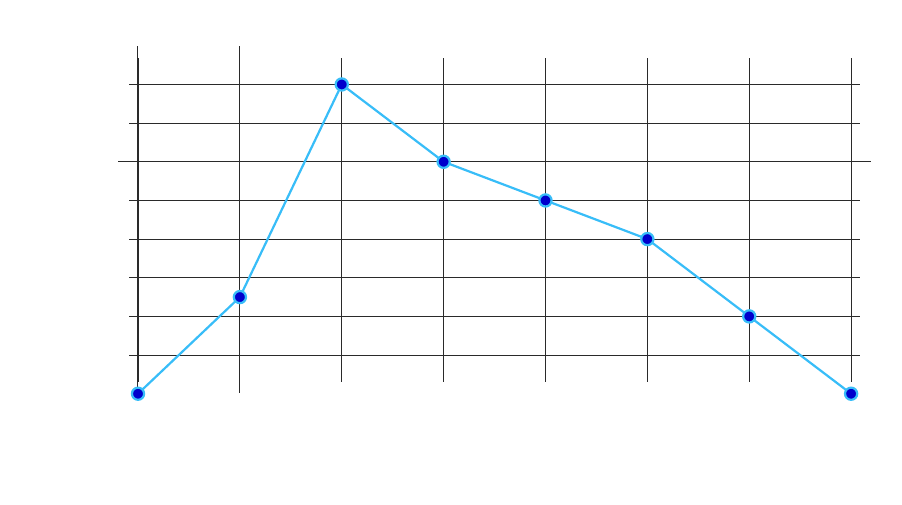
\begin{tikzpicture}
\begin{axis}[
  width=0.92\linewidth,
  height=6.0cm,
  xmin=16, xmax=53,
  ymin=0, ymax=18,
  grid=both,
  xlabel={Age (years)},
  ylabel={Frequency},
  xtick={17,22,27,32,37,42,47,52},
  ytick={0,2,4,6,8,10,12,14,16,18},
]
% Changed color to cyan so it is visible on black background
\addplot+[thick, color=cyan, mark=*, mark size=2.2pt] coordinates
{(17,0) (22,5) (27,16) (32,12) (37,10) (42,8) (47,4) (52,0)};
\end{axis}
\end{tikzpicture}
\end{center}

\end{QAPair}

% ============================================================
% Q5
\begin{QAPair}{Question 5}
\textcolor{gold}{\bfseries Question:} Represent the following data by a histogram.\\[4pt]
\begin{center}
\DarkTable
\begin{tabular}{>{\bfseries}c c c c c}
\rowcolor{tablehead}\textcolor{text}{Class interval} & \textcolor{text}{$0$--$5$} & \textcolor{text}{$5$--$15$} & \textcolor{text}{$15$--$30$} & \textcolor{text}{$30$--$40$} & \textcolor{text}{$40$--$45$}\\
\textcolor{text}{Frequency} & $5$ & $12$ & $16$ & $10$ & $2$\\
\end{tabular}
\end{center}
\tcblower
\textcolor{green}{\bfseries Answer:}

\textcolor{muted}{Since class widths are not all equal, use frequency density: $\text{FD}=f/\text{width}$.}

\[
\begin{aligned}
0\text{--}5 &: \text{width }5,\;\text{FD}=\frac{5}{5}=1.00\\
5\text{--}15 &: \text{width }10,\;\text{FD}=\frac{12}{10}=1.20\\
15\text{--}30 &: \text{width }15,\;\text{FD}=\frac{16}{15}\approx 1.07\\
30\text{--}40 &: \text{width }10,\;\text{FD}=\frac{10}{10}=1.00\\
40\text{--}45 &: \text{width }5,\;\text{FD}=\frac{2}{5}=0.40
\end{aligned}
\]

\textcolor{gold}{\bfseries Histogram (using frequency density)}\\
\begin{center}
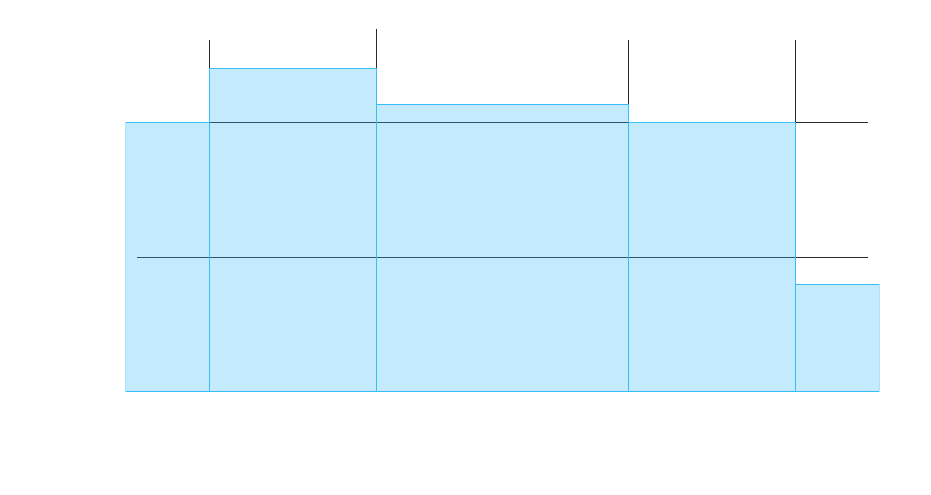
\begin{tikzpicture}
\begin{axis}[
  width=0.92\linewidth,
  height=6.2cm,
  ymin=0, ymax=1.35,
  xmin=0, xmax=45,
  grid=both,
  xlabel={Class interval},
  ylabel={Frequency density},
  xtick={0,5,15,30,40,45},
]
\addplot+[ybar interval, draw=cyan, fill=cyan, fill opacity=0.30, mark=no]
coordinates {(0,1.00) (5,1.20) (15,1.0667) (30,1.00) (40,0.40) (45,0)};
\end{axis}
\end{tikzpicture}
\end{center}

\end{QAPair}

% ============================================================
% Q6
\begin{QAPair}{Question 6}
\textcolor{gold}{\bfseries Question:} In a saving group, there are $400$ members. The number of saving certificates held is:\\
Construct a histogram of the distribution.\\[6pt]
\begin{center}
\DarkTable
\begin{tabular}{>{\bfseries}c c c c c c c}
\rowcolor{tablehead}\textcolor{text}{Class interval} &
\textcolor{text}{$1$--$50$} &
\textcolor{text}{$51$--$100$} &
\textcolor{text}{$101$--$150$} &
\textcolor{text}{$151$--$200$} &
\textcolor{text}{$201$--$300$} &
\textcolor{text}{$301$--$400$} &
\textcolor{text}{$401$--$500$}\\
\textcolor{text}{No. of members} &
$10$ & $15$ & $30$ & $40$ & $120$ & $100$ & $85$\\
\end{tabular}
\end{center}
\tcblower
\textcolor{green}{\bfseries Answer:}

\textcolor{muted}{Widths are not all equal, so use frequency density $\text{FD}=f/\text{width}$.}

\[
\begin{aligned}
1\text{--}50 &: \text{width }50,\; \text{FD}=\frac{10}{50}=0.20\\
51\text{--}100 &: \text{width }50,\; \text{FD}=\frac{15}{50}=0.30\\
101\text{--}150 &: \text{width }50,\; \text{FD}=\frac{30}{50}=0.60\\
151\text{--}200 &: \text{width }50,\; \text{FD}=\frac{40}{50}=0.80\\
201\text{--}300 &: \text{width }100,\; \text{FD}=\frac{120}{100}=1.20\\
301\text{--}400 &: \text{width }100,\; \text{FD}=\frac{100}{100}=1.00\\
401\text{--}500 &: \text{width }100,\; \text{FD}=\frac{85}{100}=0.85
\end{aligned}
\]

\textcolor{gold}{\bfseries Histogram (using frequency density)}\\
\begin{center}
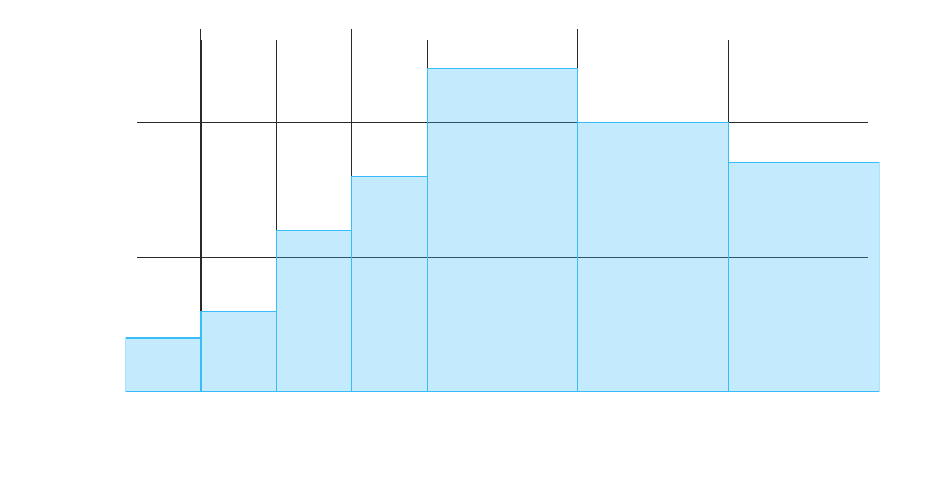
\begin{tikzpicture}
\begin{axis}[
  width=0.92\linewidth,
  height=6.2cm,
  ymin=0, ymax=1.35,
  xmin=0, xmax=500,
  grid=both,
  xlabel={Certificates},
  ylabel={Frequency density},
  xtick={0,50,100,150,200,300,400,500},
]
\addplot+[ybar interval, draw=cyan, fill=cyan, fill opacity=0.30, mark=no]
coordinates {(0,0.20) (50,0.30) (100,0.60) (150,0.80) (200,1.20) (300,1.00) (400,0.85) (500,0)};
\end{axis}
\end{tikzpicture}
\end{center}

\end{QAPair}

% ============================================================
% Q7
\begin{QAPair}{Question 7}
\textcolor{gold}{\bfseries Question:} The given frequency polygon represents per-capita income (in thousand dollars) of some states. Answer (i)--(vi).\\
\tcblower
\textcolor{green}{\bfseries Answer:}

\textcolor{muted}{Reading the points from the graph:}
\[
(10,8),\ (12,9),\ (14,13),\ (16,10),\ (18,5),\ (20,2),\ (22,1).
\]

\textcolor{gold}{\bfseries (i) Total number of states}\\
\[
\Step{1}\; 8+9+13+10+5+2+1 = 48.
\]
So, total states $= \textbf{48}$.

\textcolor{gold}{\bfseries (ii) States with the least per-capita income}\\
Least income corresponds to $10$ (thousand dollars), frequency $=8$.\\
So, \textbf{$8$ states}.

\textcolor{gold}{\bfseries (iii) States with the highest per-capita income}\\
Highest shown income is $22$ (thousand dollars), frequency $=1$.\\
So, \textbf{$1$ state}.

\textcolor{gold}{\bfseries (iv) Percent of states with income \$14000 and \$16000}\\
\[
\Step{1}\; f(14)=13,\ f(16)=10 \Rightarrow 13+10=23.\\
\Step{2}\; \%=\frac{23}{48}\times 100 \approx 47.92\%.
\]
So, approximately \textbf{$47.92\%$} (about $48\%$).

\textcolor{gold}{\bfseries (v) States with income \$18000 and above}\\
\[
\Step{1}\; f(18)+f(20)+f(22)=5+2+1=8.
\]
So, \textbf{$8$ states}.

\textcolor{gold}{\bfseries (vi) Frequency table for the polygon}\\
\begin{center}
\DarkTable
\begin{tabular}{>{\bfseries}c c}
\rowcolor{tablehead}\textcolor{text}{Per-capita income (thousand \$)} & \textcolor{text}{No. of states}\\
$10$ & $8$\\
$12$ & $9$\\
$14$ & $13$\\
$16$ & $10$\\
$18$ & $5$\\
$20$ & $2$\\
$22$ & $1$\\
\rowcolor{tablehead}\textcolor{text}{Total} & \textcolor{text}{\bfseries 48}\\
\end{tabular}
\end{center}

\textcolor{gold}{\bfseries (Diagram remake of the frequency polygon)}\\
\begin{center}
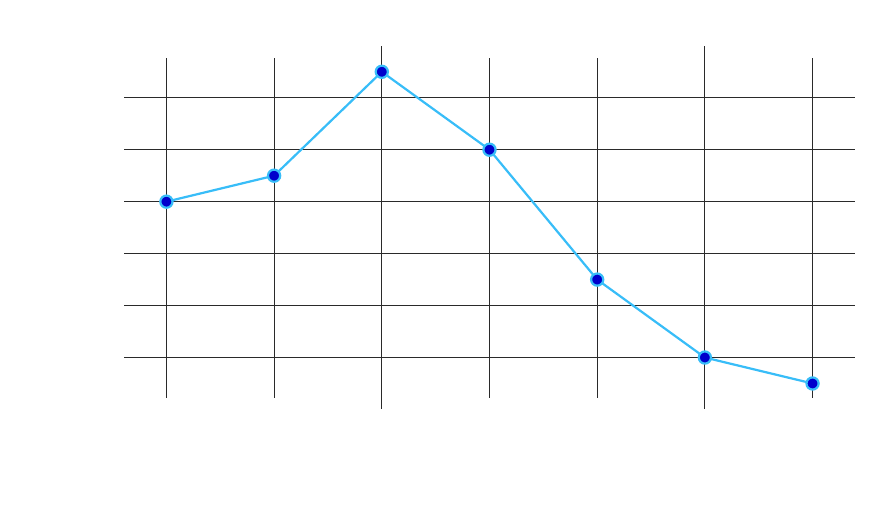
\begin{tikzpicture}
\begin{axis}[
  width=0.92\linewidth,
  height=6.2cm,
  xmin=9, xmax=23,
  ymin=0, ymax=14,
  grid=both,
  xlabel={Per-capita income (thousand dollars)},
  ylabel={Number of states},
  xtick={10,12,14,16,18,20,22},
  ytick={0,2,4,6,8,10,12,14},
]
% Changed color to cyan so it is visible on black background
\addplot+[thick, color=cyan, mark=*, mark size=2.2pt] coordinates
{(10,8) (12,9) (14,13) (16,10) (18,5) (20,2) (22,1)};
\end{axis}
\end{tikzpicture}
\end{center}

\end{QAPair}

% ============================================================
% Q8
\begin{QAPair}{Question 8}
\textcolor{gold}{\bfseries Question:} Masses (kg) of $50$ boys are given in a frequency distribution.\\
(i) Construct a histogram. \quad (ii) Construct a frequency polygon.\\[6pt]
\begin{center}
\DarkTable
\begin{tabular}{>{\bfseries}c c c c c c}
\rowcolor{tablehead}\textcolor{text}{Mass (kg)} &
\textcolor{text}{$60$--$64$} &
\textcolor{text}{$65$--$69$} &
\textcolor{text}{$70$--$79$} &
\textcolor{text}{$80$--$89$} &
\textcolor{text}{$90$--$94$} &
\textcolor{text}{$95$--$99$}\\
\textcolor{text}{Frequency $f$} &
$2$ & $6$ & $12$ & $14$ & $10$ & $6$\\
\end{tabular}
\end{center}
\tcblower
\textcolor{green}{\bfseries Answer:}

\textcolor{muted}{Widths are not equal, so for histogram use frequency density $\text{FD}=f/\text{width}$.}
\[
\begin{aligned}
60\text{--}64 &: \text{width }5,\ \text{FD}=2/5=0.40\\
65\text{--}69 &: \text{width }5,\ \text{FD}=6/5=1.20\\
70\text{--}79 &: \text{width }10,\ \text{FD}=12/10=1.20\\
80\text{--}89 &: \text{width }10,\ \text{FD}=14/10=1.40\\
90\text{--}94 &: \text{width }5,\ \text{FD}=10/5=2.00\\
95\text{--}99 &: \text{width }5,\ \text{FD}=6/5=1.20
\end{aligned}
\]

\textcolor{gold}{\bfseries (i) Histogram (frequency density)}\\
\begin{center}
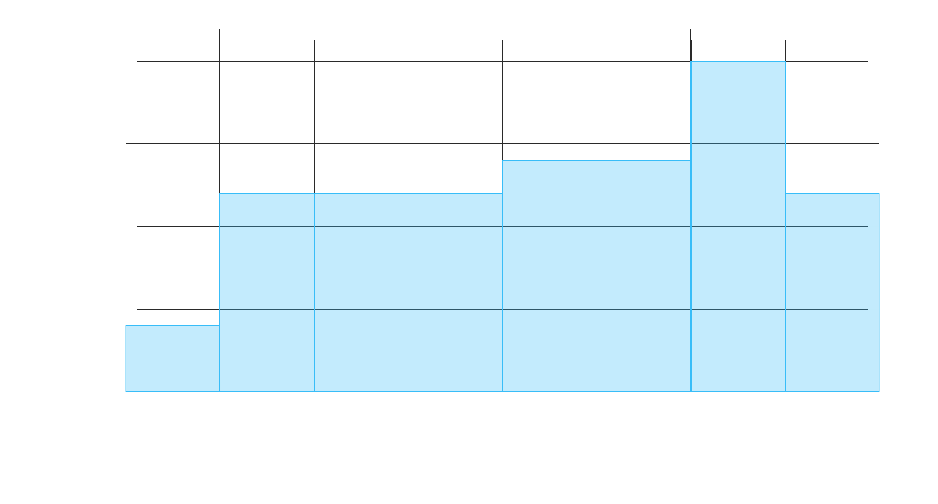
\begin{tikzpicture}
\begin{axis}[
  width=0.92\linewidth,
  height=6.2cm,
  ymin=0, ymax=2.2,
  xmin=60, xmax=100,
  grid=both,
  xlabel={Mass (kg)},
  ylabel={Frequency density},
  xtick={60,65,70,80,90,95,100},
]
\addplot+[ybar interval, draw=cyan, fill=cyan, fill opacity=0.30, mark=no]
coordinates {(60,0.40) (65,1.20) (70,1.20) (80,1.40) (90,2.00) (95,1.20) (100,0)};
\end{axis}
\end{tikzpicture}
\end{center}

\textcolor{gold}{\bfseries (ii) Frequency polygon (using the same FD heights)}\\
\textcolor{muted}{Use class marks: $62,\ 67,\ 74.5,\ 84.5,\ 92,\ 97$. Add ends with $0$.}\\
\begin{center}
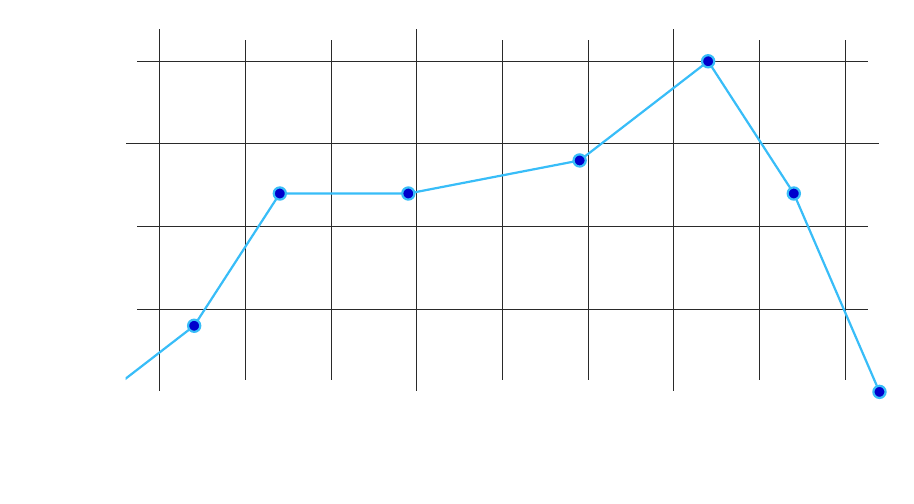
\begin{tikzpicture}
\begin{axis}[
  width=0.92\linewidth,
  height=6.2cm,
  xmin=58, xmax=102,
  ymin=0, ymax=2.2,
  grid=both,
  xlabel={Mass (kg)},
  ylabel={Frequency density},
]
% Changed color to cyan so it is visible on black background
\addplot+[thick, color=cyan, mark=*, mark size=2.2pt] coordinates
{(57,0) (62,0.40) (67,1.20) (74.5,1.20) (84.5,1.40) (92,2.00) (97,1.20) (102,0)};
\end{axis}
\end{tikzpicture}
\end{center}

\end{QAPair}

% ============================================================
% Q9
\begin{QAPair}{Question 9}
\textcolor{gold}{\bfseries Question:} At a sale, number of items placed according to the price range is given. Construct a histogram.\\[6pt]
\begin{center}
\DarkTable
\begin{tabular}{>{\bfseries}c c c c c}
\rowcolor{tablehead}\textcolor{text}{Price (Rs)} &
\textcolor{text}{$600$--$999$} &
\textcolor{text}{$1000$--$1999$} &
\textcolor{text}{$2000$--$2499$} &
\textcolor{text}{$2500$--$2999$} &
\textcolor{text}{$3000$--$3499$}\\
\textcolor{text}{Frequency $f$} &
$50$ & $70$ & $75$ & $65$ & $70$\\
\end{tabular}
\end{center}
\tcblower
\textcolor{green}{\bfseries Answer:}

\textcolor{muted}{Class widths are unequal, so use frequency density $\text{FD}=f/\text{width}$.}\\
Using continuous boundaries:
\[
\begin{aligned}
600\text{--}999 &: 599.5\text{--}999.5,\ \text{width }400,\ \text{FD}=50/400=0.125\\
1000\text{--}1999 &: 999.5\text{--}1999.5,\ \text{width }1000,\ \text{FD}=70/1000=0.070\\
2000\text{--}2499 &: 1999.5\text{--}2499.5,\ \text{width }500,\ \text{FD}=75/500=0.150\\
2500\text{--}2999 &: 2499.5\text{--}2999.5,\ \text{width }500,\ \text{FD}=65/500=0.130\\
3000\text{--}3499 &: 2999.5\text{--}3499.5,\ \text{width }500,\ \text{FD}=70/500=0.140
\end{aligned}
\]

\textcolor{gold}{\bfseries Histogram (frequency density)}\\
\begin{center}
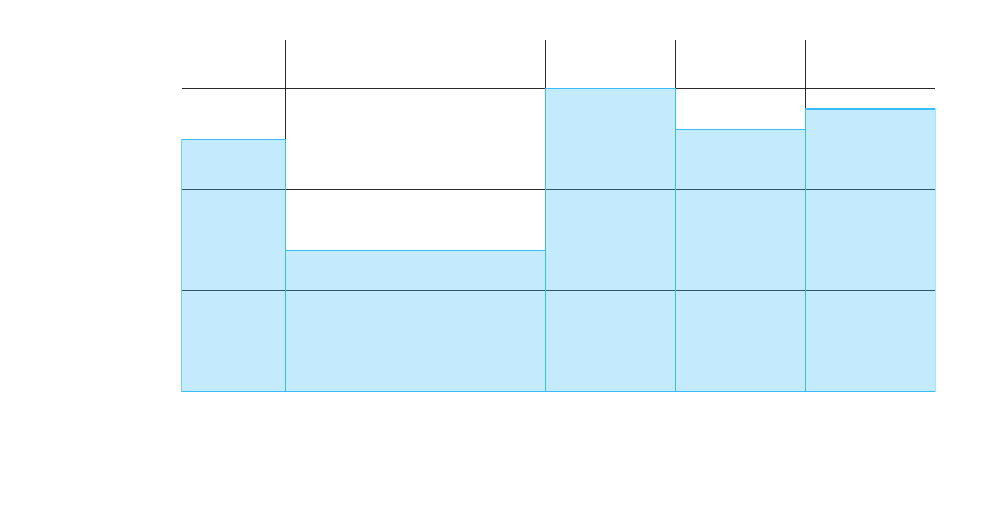
\begin{tikzpicture}
\begin{axis}[
  width=0.92\linewidth,
  height=6.2cm,
  ymin=0, ymax=0.18,
  xmin=600, xmax=3500,
  grid=both,
  xlabel={Price (Rs)},
  ylabel={Frequency density},
  xtick={600,1000,2000,2500,3000,3500},
]
\addplot+[ybar interval, draw=cyan, fill=cyan, fill opacity=0.30, mark=no]
coordinates {(600,0.125) (1000,0.070) (2000,0.150) (2500,0.130) (3000,0.140) (3500,0)};
\end{axis}
\end{tikzpicture}
\end{center}

\end{QAPair}

\end{document}